% This is samplepaper.tex, a sample chapter demonstrating the
% LLNCS macro package for Springer Computer Science proceedings;
% Version 2.21 of 2022/01/12
%

\documentclass[runningheads]{llncs}
%
\usepackage[T1]{fontenc}
% T1 fonts will be used to generate the final print and online PDFs,
% so please use T1 fonts in your manuscript whenever possible.
% Other font encondings may result in incorrect characters.
%
\usepackage{graphicx}
\usepackage{booktabs}
% Used for displaying a sample figure. If possible, figure files should
% be included in EPS format.
%
% If you use the hyperref package, please uncomment the following two lines
% to display URLs in blue roman font according to Springer's eBook style:
%\usepackage{color}
%\renewcommand\UrlFont{\color{blue}\rmfamily}
%
\begin{document}
%
\title{MALPRED: Machine Learning for Malware Prediction in Windows}
%
%\titlerunning{Abbreviated paper title}
% If the paper title is too long for the running head, you can set
% an abbreviated paper title here
%
\author{
%Le Qi Yau\inst{1} \and Mahir Hitesh Shah\inst{2} \and Eugene Jin Seng Ang\inst{1} \and Dhanvine Rameshkumar\inst{1} \and Justin Suwattana Chee\inst{3} \and Yik Ting Lam\inst{3} \and Prannaya Gupta\inst{2}
}
%
\authorrunning{
% L. Q. Yau et al.
}
% First names are abbreviated in the running head.
% If there are more than two authors, 'et al.' is used.
%
\institute{
% Temasek Junior College, 22 Bedok S Rd, Singapore 469278 \\
% \email{\{yau\_le\_qi,ang\_jin\_yew\_eugene,rameshkumar\_dhanvine\}@temasekjc.moe.edu.sg}\\
% \url{https://www.temasekjc.moe.edu.sg/} \and
% NUS High School of Mathematics and Science, 20 Clementi Ave 1, Singapore 129957 \\
% \email{\{h1910099,h1810124\}@nushigh.edu.sg} \\
% \url{https://www.nushigh.edu.sg/} \and
% Dunman High School, 10 Tanjong Rhu Rd, Singapore 436895 \\
% \email{\{chee.justin.suwattana,lam.yikting\}@dhs.edu.sg} \\
% \url{https://www.dunmanhigh.moe.edu.sg/}
}
%
\maketitle              % typeset the header of the contribution
%
\begin{abstract}
Malware infections are a pervasive issue for computers running the Windows operating system. In this study, we present a machine-learning based approach to predict the likelihood of malware infection in Windows machines. Our methodology involves conducting data pre-processing, feature engineering, and selection on the Microsoft Malware Prediction dataset. We then perform extensive experimentation using various machine learning algorithms and identify XGBoost, LightGBM and CatBoost as the 3 best-performing algorithms. Through hyperparameter tuning via the Tree-Structured Parzen Estimator and using a Meta Learner on top of our top 3 best-performing algorithms, our optimal novel model achieves an AUC score of 73.24\% across Stratified 5-fold cross-validation, demonstrating the efficacy of our approach. Additionally, we develop a web-based interface enabling users to input their Windows machine specifications and obtain predictions regarding the probability of malware infection.

\keywords{Machine Learning  \and Windows \and Malware \and Tree-Structured Parzen Estimator \and XGBoost \and LightGBM \and CatBoost \and Meta Learner.}
\end{abstract}

\section{Introduction}
\par 
The Microsoft Windows Operating System (hereby referred to as Windows OS) is one of the most widely-used operating systems in the world, with more than 1.4 billion monthly active devices and 74\% of computer users running Windows 10 or Windows 11 \cite{microsoftahaha}. Due to the widespread use, malware is often created specifically for Windows OS. Malware refers to malicious software such as viruses, worms, trojans, etc. An example is WannaCry \cite{kaspersky_2022}, a form of ransomware that infected 230,000 computers in just hours, leading to up to \$4 billion dollars of damage. It is therefore of utmost importance that there is a reliable mechanism that can advise users on the likelihood of infections and prevent malware from causing more significant issues.

\par
Malware is often analysed in three major forms: static, dynamic and a hybrid of both forms. Static analysis involves analysing static features of the malware sample, such as its strings and PE Headers, while dynamic analysis places the malware sample into a sandbox and extracts its behaviour. Machine learning is also increasingly adopted into malware analysis due to its ability to identify patterns based on large data samples. However, these methods largely focus on analysing specific malware samples, rather than the entire system.

\par
In this paper, we aim to focus on using the specifications of the Windows machine to determine the likelihood of malware infection. The contributions of this paper are as follows:
\begin{itemize}
\item  Extensive feature processing and engineering of the dataset provided in the Microsoft Malware Prediction.
\item A comprehensive set of experiments on the post-processed data set for an empirical comparison among various machine learning models, as well as building a Meta Model from the best 3 performing models
\item Hyperparameter tuning of the best models to obtain better performance.
\item A Novel Web Application Interface to access the finalised model.
\end{itemize}


\section{Related Works}

In the past, several teams have presented work aiming to use the specifications of the Windows machine. Most of these works \cite{iop2020,shahini2019,sokolov2021} utilise the Microsoft Malware Prediction dataset, publicly available on Kaggle \cite{microsoft-malware-prediction}, and most authors evaluate their models mainly on the Area under the ROC curve (hereby referred to as the AUC score).

Pan et al \cite{iop2020} preprocessed the aforementioned dataset by reducing the memory of the data (by removing largely null columns and switching data types to less precise forms), then utilised chi-square testing to evaluate the more useful metrics to the actual label. Following this, they trained 3 models on the dataset: Logistic Regression, K-Nearest Neighbours (KNN) and Light Gradient Boosting Machine (LightGBM). The team found that the LightGBM model attained a high AUC score of 0.72.

Similarly, Shahini et al \cite{shahini2019} also preprocessed the data similarly by removing largely null columns. The team then trained a LightGBM model due to its lower memory usage and faster training speed. The team attained an AUC score of 0.74. Following this, they also investigated the model to find the features that contributed the most to the model, citing \texttt{FirmwareVersionIdentifier}, \texttt{CityIdentifier},  and \texttt{SystemVolumeTotalCapacity} as the most contributive features to their model.

Sokolov et al \cite{sokolov2021} conducted a series of experiments to determine the best feature selection method. Following this, he then utilised Automated Artificial Intelligence (AutoAI) methods to evaluate the stated feature selection methods, in addition to LightGBM, Naive Bayes and Logistic Regression. Through the series of experiments, the team proposed an ensemble model composed of five different LightGBM models, each trained on a different fold of the dataset. Sokolov et al evaluated their models using the accuracy, precision, recall and $F_1$ scores and attained an accuracy score of 0.6799.

\section{Methodology}

\begin{figure}[h]
\includegraphics[scale=0.25]{images/Microsoft Malware Prediction Data Set (1350 × 800 px).png}
\centering
\caption{A simple overview of our approach}
\label{Fig 1}
\end{figure}

\subsection{Overview}
An overview of our methodology is presented in Fig.\ref{Fig 1}\footnote[1]{Icons from Pixel Perfect, Eucalyp, Paul J., Freepik, and Canva have been used when designing the figures.}. Our methodology is split into 2 phases. The first phase involves the model being trained on the Microsoft Malware Prediction dataset from Kaggle \cite{microsoft-malware-prediction}. Using the PyCaret library \cite{pycaret}, we perform extensive feature preprocessing and engineering on the dataset. We then train the hypertuned model. The second phase involves the deployment of the model on a Web Application Interface. Our Web Application User Interface (UI) allows users to input the specifications of their personal computers. Following that, inference is conducted and the probability of infection is displayed.
\subsection{Microsoft Malware Prediction Dataset}
In this paper, the Microsoft Malware Prediction Dataset from Kaggle \cite{microsoft-malware-prediction} is used. The dataset contains 8,921,483 samples, each one representing a different Windows Machine, with 83 features extracted from each machine. The \texttt{"HasDetections"} column indicates whether the Windows Machine has been previously infected by the malware. As some features have many missing values while other features are not strongly correlated to whether a Windows Machine is likely to get infected, extensive feature preprocessing and engineering is required in order to achieve good results on machine learning models. 
\subsection{Feature Engineering and Preprocessing}
\begin{figure}[h]
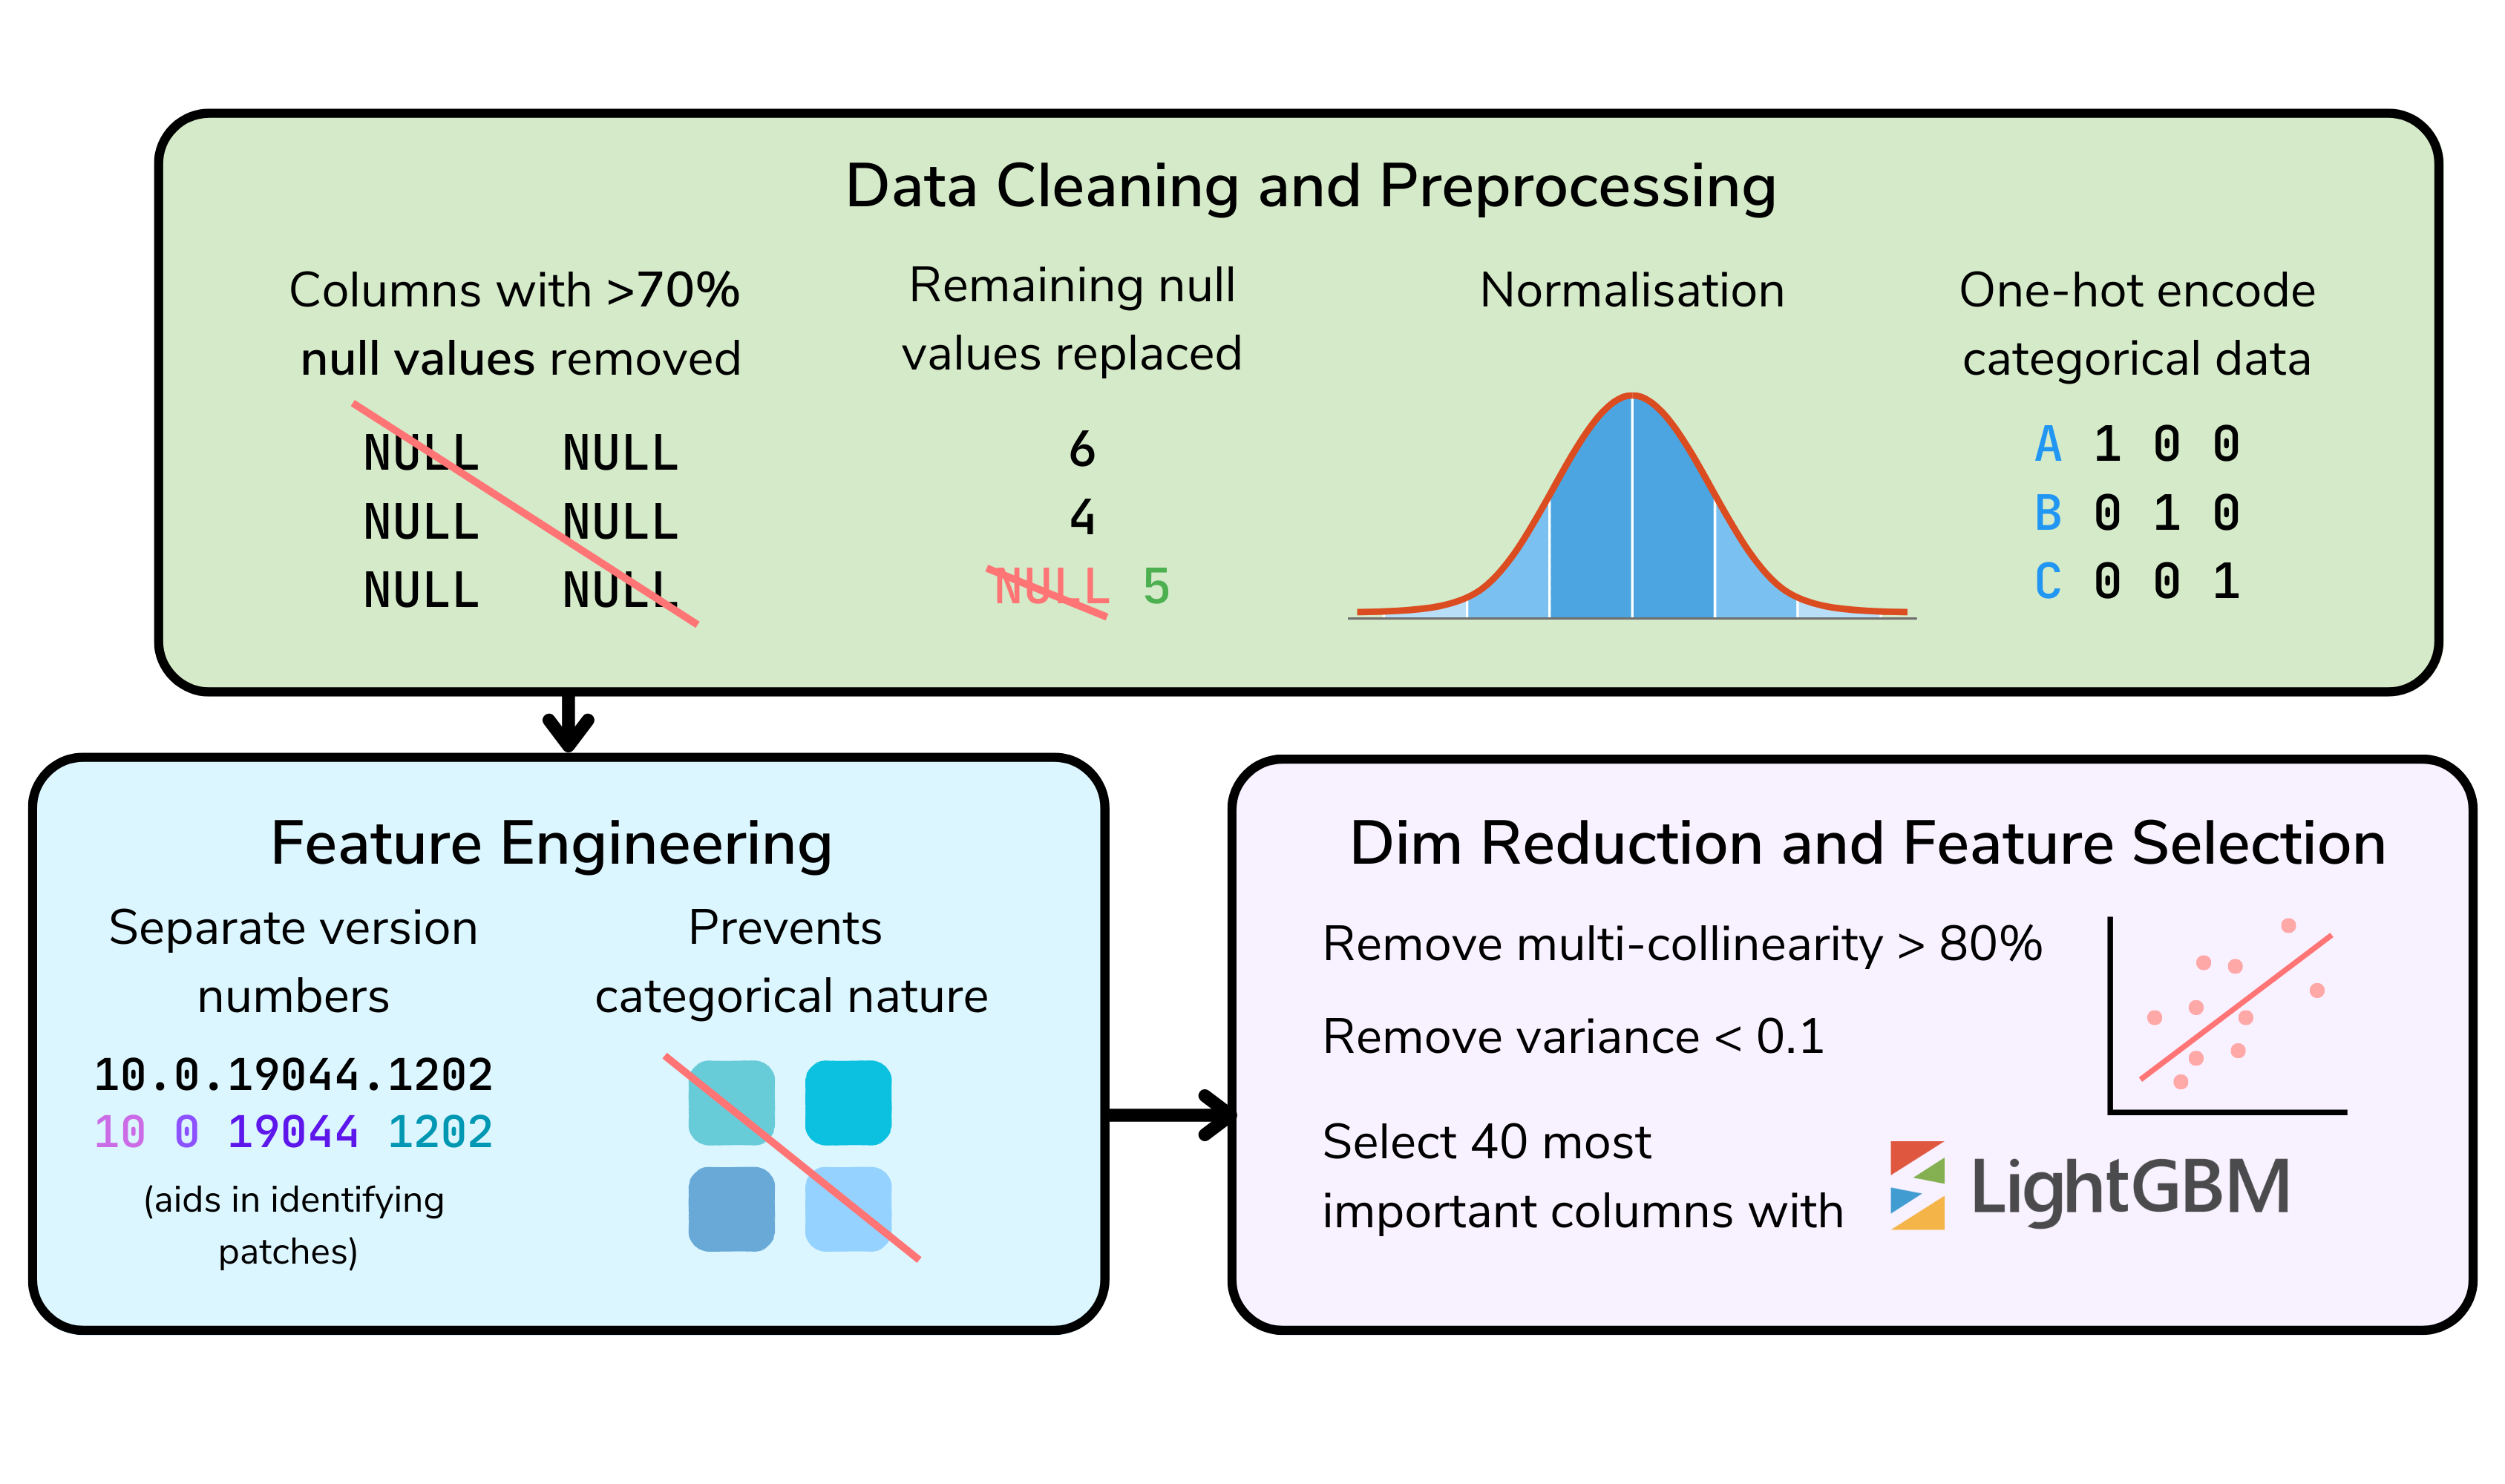
\includegraphics[scale=0.25]{images/feature_engineering.png}
\centering
\caption{Feature Engineering and Preprocessing}
\label{Fig 2}
\end{figure}
\subsubsection{Data Cleaning and Processing} 
An overview of the preprocessing is shown in Fig.\ref{Fig 2}. Firstly, similar to \cite{shahini2019}, columns with more than 70\% null values, {(specifically \texttt{PuaMode}, \texttt{Census
ProcessorClass}, \texttt{DefaultBrowsersIdentifier}, \texttt{Census Is
-FlightingInternal}, and \texttt{Census InternalBatteryType})} are noted to likely not be helpful in the task at hand and are therefore removed. For other samples that still have null values for other columns, we utilise the simple imputer found in PyCaret to replace the null values. For categorical columns, the null values are replaced by the most frequent value found in the column. For numerical columns, the null values are replaced by the mean of the column. Normalisation is also performed on numeric columns such that the difference in values for all numeric columns is not drastically different. Categorical data is one hot encoded as the machine learning model is unable to process categorical data directly.
\subsubsection{Feature Engineering} 
In the provided data set, there are 6 fields which are version identifiers. These identifiers have 4 sections separated by dots, showing the major, minor, build and patch numbers. Since the versions that are released closer together are likely to have similar security vulnerabilities, each version field was separated such that each section is a field \cite{iop2020}. This is to allow the models to see how close the versions are instead of having categorical data. This can also help us find which versions may have patches for vulnerabilities.
\subsubsection{Dimension Reduction and Feature Selection}
Before we train our models, we must first investigate the dataset for any highly correlated features, as they do not generally contribute to the performance and add to the variance of the coefficients of the model. This can lead to the model being more unstable in general, thus we remove columns where the multi-collinearity score is found to be higher than 80\%, and also columns with a variance lower than 0.1. From here, we perform Feature Selection to select the 40 most important columns using the Light Gradient Boosting Machine (LightGBM) model.
\subsection{Machine Learning Models}
We evaluate 3 different models to predict the probability of the Windows Machines being infected by Malware: Extreme Gradient Boosting Classifier (XGBoost), Cat Gradient Boosting Classifier (CatBoost), and Light Gradient Boosting Machine (LightGBM). We chose these 3 models as these 3 models are shown to have good performance when on numerical data. Other than these 3 models, we also evaluated Support Vector Machines (SVM), Decision Trees (DT), Linear Discriminant Analysis (LDA), Multilayer Perceptron (MLP), AdaBoost (ADA), Quadratic Discriminant Analysis (QDA), Gradient Boosting Classifier (GBC), Ridge Classifier (Ridge), and a Dummy Classifier (Dummy) that ignores input features, to compare the effectiveness of our model. We also introduce a novel method using a meta-learner that uses a logistic regression model as Meta Learner and learns the output of the three best-performing models.

\subsection{Hyperparameter Tuning}
We then tune the hyperparameters of the best-performing model using Tree-Structured Parzen Estimator (TPE), a novel method not highlighted in prior literature. This is because it can exploit the inherent tree structure of models such as Random Forest, Decision Trees and Gradient Boosting Classifiers. TPE balances the exploration and exploitation, efficiently handles high-dimensional spaces and uses Kernel Density Estimation (KDE) to focus on promising hyperparameter configurations, reducing computational resources as well. This led to us using TPE as the search algorithm for hyperparameter tuning.

\section{Results}

\begin{figure}[!h]
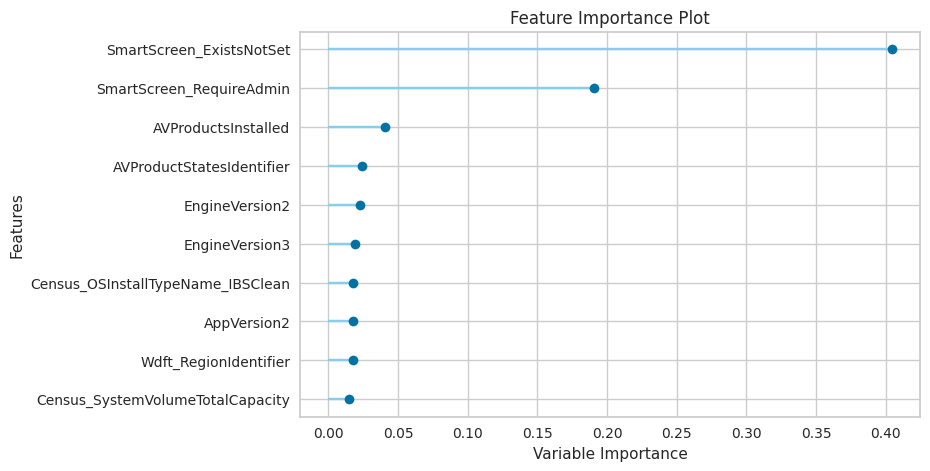
\includegraphics[scale=0.5]{images/importance.png}
\centering
\caption{Feature Importance of Top 10 fields}
\label{Fig 3}
\end{figure}

\subsection{Feature Importance} It is important to see which features play the biggest role in the decisions of the model. This is to see what improvements can be made to reduce the chance of getting infected by the malware the most. As seen in Fig 3, the top 4 features are related to the SmartScreen and Antivirus. These features protect computers from getting infected, so it makes sense that they affect the probability of a computer getting infected greatly. The top features also contain build and patch numbers. A change in these numbers normally connotes a fixed bug or possibly more bugs created by the fix, thus their high importance in the model. 
\subsection{Experimental Setup and Metrics}We evaluate the models using 5-Fold Cross Validation, where the dataset is split into 5 equal sets, and four sets are used for training the model, while one set is used for the evaluation of the model. The process is repeated until all 5 sets of data have been tested individually and the scores for each fold will be averaged. This reduces any bias in the dataset as all data in the dataset is used for testing. For metrics, we evaluate the performance of our model using Area Under Curve (AUC-ROC), Accuracy, Recall, Precision as well as the F1 score. We mainly optimised on the AUC as the focus of the classifier was to generate probabilities of malware infections. The AUC is also noted to be the main metric evaluated from Microsoft as noticed from the Kaggle competition \cite{microsoft-malware-prediction}. 

%This is likely to be more helpful in the task at hand, as we want to maximize the AUC score, to ensure that our classifier can accurately predict the probability of the Windows Machine being infected by malware as much as possible. 
% \iffalse
% \begin{table}
%     \centering
%     % \setlength{\tabcolsep}{17pt} % Adjust the column separation
%     % \renewcommand{\arraystretch}{1.5} % Adjust the row spacing
%     \begin{tabular}{cc}
%         \toprule \textbf{Metric} & \textbf{Formula for Computation} \\
%         % \midrule $F_1$ Score & $$\frac{2 \cdot TP}{2 \cdot TP + FN + FP}$$ \\
%         Accuracy Score & $a = \frac{TP+TN}{TP+TN+FP+FN}$ \\
%        \bottomrule
%     \end{tabular}
%     \caption{Visual Representation of metrics used, where TP: True Positive, FP: False Positive, TN: True Negative, FN: False Negative}
%     \label{tab:my_label}
% \end{table}


% \begin{table}
%     \centering
%     \setlength{\tabcolsep}{17pt} % Adjust the column separation
%     \renewcommand{\arraystretch}{1.5} % Adjust the row spacing
%     \begin{tabular}{ |p{5cm}|p{4cm}| }
%     \hline
%     Equation & Description \\ \hline
%     $$Fn = \frac{(1 + B^2)TP}{(1 + B^2)TP + B^2 \cdot FN + FP}$$ & Fn Score \\ \hline
%     $Accuracy = \frac{TP+TN}{TP+TN+FP+FN}$ & Accuracy \\ \hline
%     $AUC = \text{Area Under the Curve}$ & AUC (Area Under the Curve) \\ \hline
%     \end{tabular}
%     \newline
%     \newline
%     \caption{Visual Representation of metrics used, where TP: True Positive, FP: False Positive, TN: True Negative, FN: False Negative, B: relative importance of recall over precision \cite{}}
%     \label{table:Table1}
% \end{table}
% \fi
\subsection{Experiments with Machine Learning Models}
As shown in Table \ref{tab:allaimodels}, the stack model performed the best amongst all models. The Ridge and SVM also do not have AUC-ROC as they do not generate probabilities.
\begin{table*}
\centering
\caption{Score of Machine Learning Models over 5-fold Cross Validation (Best results bolded)}
\label{tab:allaimodels}
\begin{tabular}{@{}lcccccc@{}}
\toprule
 {\bf Models} & {\bf AUC-ROC} & {\bf Accuracy} & {\bf Recall} & {\bf Precision} \\ \midrule %\hline\hline
 \textbf{Stack Model} & $\mathbf{73.03}$ & $\mathbf{66.45}$ & $\mathbf{66.25}$ & $\mathbf{66.49}$ \\ 
XGBoost & $72.19$ & $65.79$ & $65.18$ & $65.96$ \\
LightGBM & $71.25$ & $65.08$ & $64.21$ & $65.33$ \\ 
CatBoost & $70.92$ & $64.78$ & $63.50$ & $65.15$ \\ 
MLP & $70.72$ & $64.62 $ & $63.56$ & $64.94$ \\ 
GBC & $69.50$ & $63.57 $ & $64.22$ & $63.38$ \\ 
ADA & $68.75$ & $63.14$ & $64.87$ & $62.68$ \\ 
LDA & $66.72$ & $61.68$ & $57.79$ & $62.64$ \\ 
QDA & $66.23$ & $56.98$ & $65.85$ & $61.51$ \\ 
DT & $57.60$ & $57.60$ & $57.73$ & $57.56$ \\ 
Dummy & $50.00$ & $50.02$ & $00.00$ & $00.00$ \\ 
Ridge & $-$ & $61.68$ & $57.79$ & $62.64$ \\
SVM & $-$ & $61.34$ & $51.93$ & $63.97$ \\ \bottomrule
\end{tabular}%
\vspace{-1ex}
\end{table*}

\subsection{Experiments with Hypertuning}
Due to our limited resources, we extracted 10\% of the dataset, then utilised the TPE algorithm using PyCaret \cite{pycaret} to tune our model with 100 iterations. We tuned XGBoost, CatBoost and LightGBM using the TPE method. However, the TPE tuning did not return a better model when compared to the LightGBM, as such, we did not include LightGBM in the results below. We then take the best parameters derived from the hypertuning and apply them to our models to test on the whole dataset. We also reconstructed the Meta Model, with the tuned XGBoost \cite{Chen:2016:XST:2939672.2939785}, CatBoost \cite{cat} and the original LightGBM \cite{ke2017lightgbm}, and the tuned XGBoost as a Meta Learner. 
\begin{table*}
\centering
\caption{Comparison of tuned and untuned models (in percentage)}
\label{tab:allaimodels}
\begin{tabular}{@{}lcccccc@{}}
\toprule %\hline
 {\bf Models} & {\bf AUC-ROC} & {\bf Accuracy} & {\bf Recall} & {\bf Precision} \\ \midrule %\hline\hline
XGBoost & $72.19$ & $65.79$ & $65.18$ & $65.96$ \\ %\hline
 XGBoost (TPE Tuned) & $72.95$ & $64.95$ & $\mathbf{80.58}$ & $61.38$ \\ \hline
Normal CatBoost & $70.92$ & $64.78$ & $63.50$ & $65.15$ \\ %\hline
 CatBoost (TPE Tuned) & $72.37$ & $65.95$ & $65.11$ & $66.20$ \\ \hline
 Normal Stacked & $73.03$ & $\mathbf{66.45}$ & $66.25$ & $\mathbf{66.49}$ \\ %\hline
 Stacked (TPE Tuned) & $\mathbf{73.24}$ & $65.36$ & $79.81$ & $61.90$ \\ \bottomrule %\hline
\end{tabular}%
\vspace{-2ex}
\end{table*}

\subsection{Discussion of Results}
As expected, the gradient boosting models, such as XGBoost, LightGBM and CatBoost, had the best performance on the dataset. MLP is shown to have the next best performance, therefore suggesting the effectiveness of a deep learning approach. Our Meta Model is shown to have the best performance among the untuned models, with the highest AUC score of 73.03\%. The TPE tuning also improved the performance of most of our models, with our models seeing an improvement of up to 1.45\% in the AUC score. Our finalised model, the TPE-tuned Meta Model, with an AUC score of 73.24\% outperforms most existing works, and is only a stone's throw away from the State of The Art (SOTA) model \cite{shahini2019}, which achieved 74\% AUC over 5-Fold Cross-Validation. However, we believe that given more resources, we could have performed TPE tuning across the entire dataset, and matched or even exceed the performance of the SOTA model. 

\subsection{Web Application}
We used PyCaret to create a Gradio \cite{gradio} app interface for our web application. Gradio is a free and open-source Python library that allows us to develop an easy-to-use customisable component demo for our machine learning model. The novel web app takes in several parameters as inputs and returns the probability of the presence of malware. The Web Application User Interface can be seen in \ref{fig:enter-label}.
\begin{figure}
    \centering
    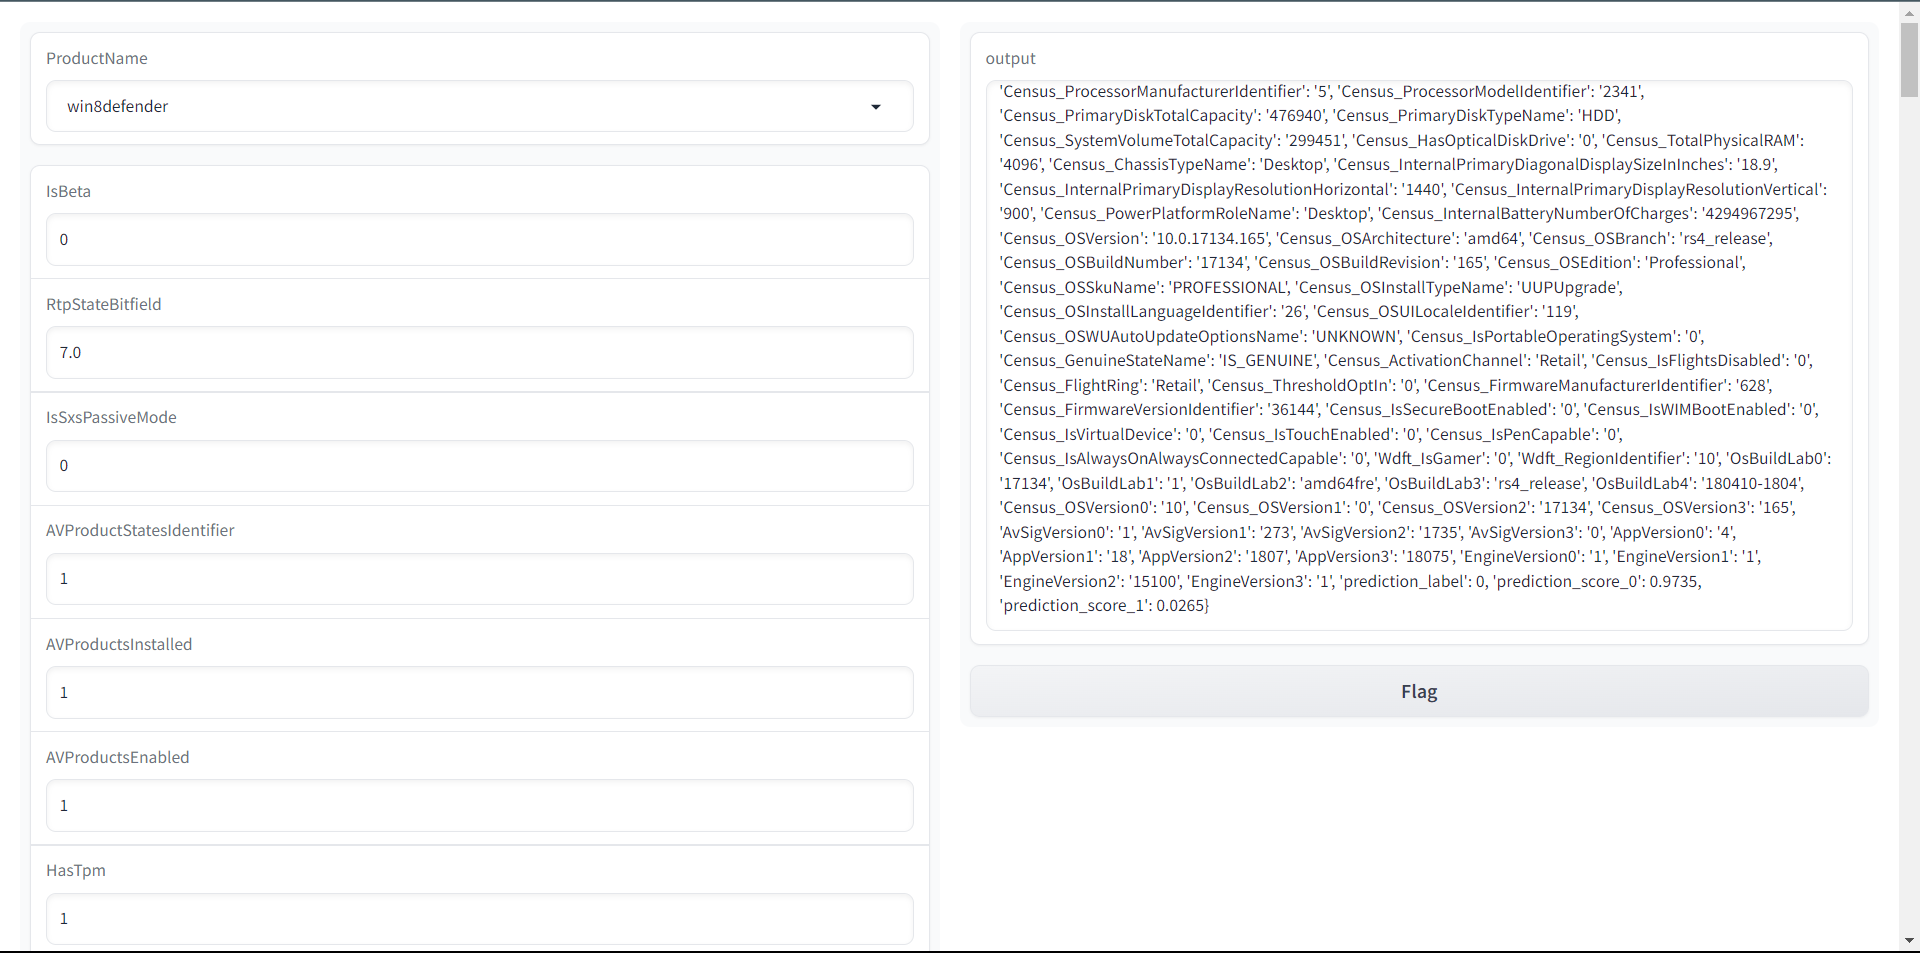
\includegraphics[width=\linewidth]{images/Gradio App Screenshot.png}
    \caption{Gradio Web Application User Interface}
    \label{fig:enter-label}
\end{figure}

\section{Conclusion}
In this paper, we proposed a method of data cleaning, feature engineering and feature selection for the Microsoft Malware Dataset. We test our feature processing method using various models, such as XGBoost, Cat Boost and LightGBM. We than stack the models together and use a Meta Learner which learns from the output of the best 3 performing models. Finally, we perform hyperparameter tuning using the Tree-Structured Parzen Estimator method. Our model achieves a AUC score of 73.24\%. 

% \subsection{Future Works}
In the future, we wish to explore the use of Large Language Models (LLMs) on this dataset. We also hope to obtain newer data regarding for this, as the Microsoft Malware Dataset dates back to 2015, where most people were using Windows 8.1. Finally, we hope to develop a desktop application that can automatically collect the specifications of the machine before sending it to the API for inference. 







\bibliographystyle{splncs04}
\bibliography{bib}



\end{document}